\documentclass[12pt]{article}
\usepackage{graphicx}
\usepackage{fullpage}
\usepackage{verbatim}
\usepackage{caption}
\usepackage{float}
\usepackage[nottoc]{tocbibind} 
\usepackage{appendix}
\usepackage{titlesec}
\usepackage{tikz}
\usepackage{listings}
\usepackage{hyperref}
\hypersetup{
    colorlinks=true,
    linkcolor=blue,
    filecolor=magenta,      
    urlcolor=blue,
}
\usepackage[utf8]{inputenc}
\urlstyle{same}
\usetikzlibrary{shapes,arrows}
\titleformat{\chapter}[display]
  {\normalfont\bfseries}{}{0pt}{\Large}
  \usepackage[T1]{fontenc}
\usepackage[utf8]{inputenc}

  


\begin{document}
  \begin{titlepage}
    \begin{center}
      \begin{Large}
      \textbf{ Assignment- 8\\
       \vspace*{0.5cm}
       ELP - 718 Telecom Software Laboratory\\
       \vspace{1cm}
       Ch Krishna Chaitanya\\
       2019JTM2674\\
       2019-21\\}
      \end{Large}
       \vspace{1cm}
      {\Large  A report on Python Basics}
       \vfill
       \begin{figure}[h!]
          \centering
          
\includegraphics{iitdelhi.png}
       \end{figure}
       \vfill
      \begin{Large}
      \textbf{ Bharti School of \\
       Telecommunication Technology and Management\\
       IIT Delhi\\
       India\\
      }\end{Large}
       \medskip
       \today
    \end{center}
    \vfill
  \end{titlepage}
  
  \tableofcontents
  
  \clearpage
  \section*{Objective Statement}
   To Test our understanding of python basics including lists and functions.

  \section{Problem Statement -1}
 To write a python program to find simplest way of error detection and to append a single bit, called a parity check, to a string of data bits
  \subsection{Problem Satement}
  
  \subsection{Algorithm and Implementation}
  \begin{itemize}
  \item Enter Input
  \item Check Parity
  \item Print data after parity check
  \item Find substring
  \item Append 0 after substring
  \item Append 0101 to indicate end of frame
  \end{itemize}
  \subsection{Flowchart}
    % Define block styles
\tikzstyle{decision} = [diamond, draw, fill=blue!20, 
    text width=4.5em, text badly centered, node distance=3cm, inner sep=0pt]
\tikzstyle{block} = [rectangle, draw, fill=blue!20, 
    text width=6.5em, text centered, rounded corners, minimum height=3em]
\tikzstyle{line} = [draw, -latex']
\tikzstyle{cloud} = [draw, ellipse,fill=red!20, node distance=3cm,
    minimum height=3em]
\begin{center}    
\begin{tikzpicture}[node distance = 2cm, auto]
    % Place nodes
    
    \node [cloud] (init) {start};
    \node [block, below of=init] (First) {Enter Bit string};
    \node [block, below of=First] (Second) {Find number 0f 1's};
    \node [decision, below of=Second] (decide) {Check odd or even};
     \node [block, below of=decide,node distance=3cm] (Staff) {Append 0,Bit stuff,flag bits};
     \node [block, left of=decide,node distance=4cm] (Customer) {Append 1};
     
    \node [block, below of=Customer,node distance=3cm] (cust_des) {Bit stuffing and flag bits};
    \node [block, below of=cust_des] (stop_cust) {stop};
    \node [block, below of=Staff] (stop_st) {stop};
  
    
    % Draw edges
    \path [line] (init) -- (First);
    \path [line] (First) -- (Second);
    \path [line] (Second) -- (decide);
     \path [line] (decide) --(Staff);
     \path [line] (Staff) --(stop_st);
     \path [line] (decide) --(Customer);
     \path [line] (Customer) --(cust_des);
     \path [line] (cust_des) --(stop_cust);
     
    
   
\end{tikzpicture}
\end{center}
  \subsection{Input and Output format}
  \subsubsection{Input Format} 
Enter binary bit data that has to be transmitted.\\


\subsubsection{Output Format}
Print binary bit data with parity bit.\\
Print the modified string that is to be transmitted\\

  \subsection{Test Cases}
  \subsubsection{Input1}
  010101110100101\\

    
  \subsubsection{Output1}
  Parity bit data : 0101011101001011\\
Transmitting data: 01001011101000100110101\\

\subsection{Screenshots}
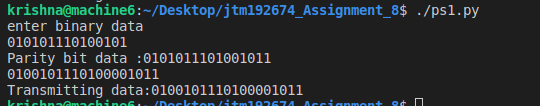
\includegraphics[width=\linewidth]{lab8_1.png}
  \section{Problem Statement -2}
  \subsection{Problem Satement}
   To write a python program for a 3X3 tic tac toe.


  \subsection{Algorithm and Implementation}
  \begin{itemize}
  \item Check if player want to enter odd number
  \item Player1 enters choice
  \item Enter number and position between 0-9
  \item Player2 enters choice
  \item Enter number and position between 0-9
  \item Check if sum in a row or column or diagonal > 15
  \item If > 15, Gameover
  \end{itemize}
  \subsection{Flowchart}
    % Define block styles
  \tikzstyle{decision} = [diamond, draw, fill=blue!20, 
    text width=4.5em, text badly centered, node distance=3cm, inner sep=0pt]
\tikzstyle{block} = [rectangle, draw, fill=blue!20, 
    text width=6.5em, text centered, rounded corners, minimum height=3em]
\tikzstyle{line} = [draw, -latex']
\tikzstyle{cloud} = [draw, ellipse,fill=red!20, node distance=3cm,
    minimum height=3em]
  \begin{center}    
\begin{tikzpicture}[node distance = 2cm, auto]
    % Place nodes
    
    \node [cloud] (init) {start};
    \node [block, below of=init] (First) {Player1,s Chance};
    \node [block, below of=First] (Second) {Enter position and number};
    \node [block, below of=Second] (Third) {Player2,s Chance};
    \node [block, below of=Third] (Fourth) {Enter position and number};
    \node [block, below of=Fourth] (Fifth) {Check if>15};
    \node [block, below of=Fifth] (Sixth) {Stop};
 
    
    
    % Draw edges
    \path [line] (init) -- (First);
    \path [line] (First) -- (Second);
    \path [line] (Second) -- (Third);
     \path [line] (Third) -- (Fourth);
    \path [line] (Fourth) -- (Fifth);
    \path [line] (Fifth) -- (Sixth);
  
   
    
\end{tikzpicture}
\end{center}
  
 \newpage
  \subsection{Test Cases}
  \subsubsection{Constraints}
  1<=Position<=9\\
1<=Number<=9\\


	\subsubsection{Input}
	Print ‘Welcome to the Game!’. \\   
Print whether it is Player 1’s or Player 2’s chance.\\
Get the position and number to be entered from the user.\\
Show tic tac toe with data.\\
Continue till the game gets draw or some player wins and show the result.\\
Ask the user whether to continue for the next game or exit.\\
\subsubsection{Output}
Welcome to the Game\\
Player 1's chance\\
Enter the position and number to be entered:1 5
0 0\\
5 0 0\\
0 0 0\\
0 0 0\\
2\\
Player 2’s chance\\
Enter the position and number to be entered:5 6\\
1 1\\
5 0 0\\
0 6 0\\
0 0 0\\
Continue
\subsection{Screenshots}
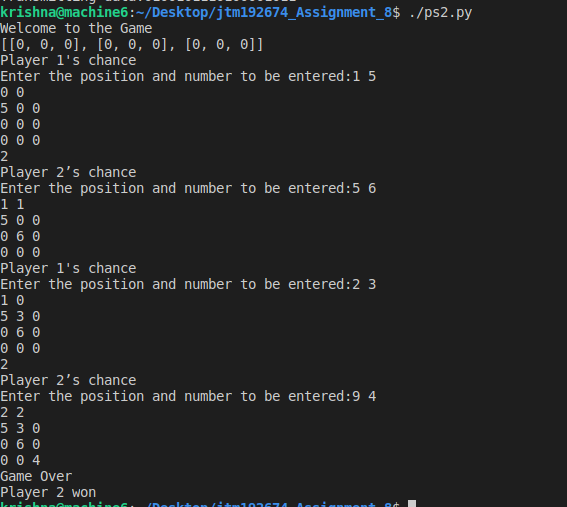
\includegraphics[width=\linewidth]{lab8_2.png}

 \appendix
   \appendixpage
   \addappheadtotoc
  \section*{Problem 1}
  {\large \textbf{code:}}
  \verbatiminput{ps1.py}
  \section*{Problem 2}
  {\large \textbf{code:}}
  \verbatiminput{ps2.py}
  
  
\newpage
\begin{thebibliography}{11}
\bibitem{flowchart} 
Flowchart using Latex\\
Kjell Magne Fauske \\
\url{http://www.texample.net/tikz/examples/simple-flow-chart/}

\bibitem{Python Basics}
Python Basics \\
\url{https://docs.python.org/3/}

\bibitem{Python Examples}
Python Examples\\
\url{https://www.geeksforgeeks.org/python-list/}

\bibitem{Git Hub}
Git Hub\\
\url{https://help.github.com/en/articles/fork-a-repo}

\bibitem{Python regular expressions}
Python regular expressions\\
\url{https://docs.python.org/3/howto/regex.html}

\end{thebibliography}


  
   
   
\end{document}
